\chapter{Implementation}
This chapter serves to discuss the implementation specifics of the design of my application, including the development environment and any issues I encountered in implementing the features set out in my project objectives.

\section{Development Environment}
The application was developed primarily on a Fujitsu Lifebook A series with an Intel i5-3230M CPU @ 2.60GHz processor, 4GB of RAM and running Windows 10. The code was developed using Jet Brains IntelliJ IDE and Google Chrome developer console.

\section{Features}
\subsection{Reading User Input}
\subsubsection{Implementation}
The user input was one of the first parts of the application to be implemented, and consisted of reading in a .fa FASTA file and just outputting the content of the file to the console and return it from the method to be tested against with automated unit tests. It was developed further to extract out the header, checking that it began with the `\textgreater ' character and then every other line was included as part of that contig. 

Originally it dealt with only one contig at a time, but was then expanded to be able to read in a full list of contigs and separate them based on where the header line starts. The code was eventually modified so that the user could paste data, that would be broken into components and processed in the same way. This was for the pasting of the user data rather than file upload, as I decided I would rather have pasted data than uploads for the current state of the application.

\begin{figure}[H]
\centering
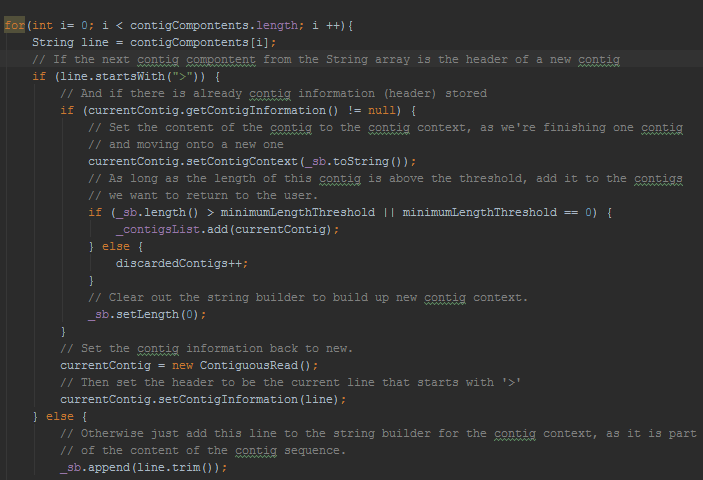
\includegraphics[width=0.8\textwidth]{images/readuserdata}
\caption{Part of the code for reading in a users data when they have pasted it into the text area of the web service. Deals with creating new ContiguousRead objects and adding them to a ContigResult every time it finds a new header for a contig (or reaches the end of the input).}
\end{figure}

\subsubsection{Issues}
I found during implementation of the reading user data that there weren't that many issues. It took some time to deal with the formatting of the file and knowing when one contiguous read starts and one ends. There was some issue with the escape/return characters in the dealing of pasted content by a user, but this was solved by breaking the pasted content into an array of its components.

While not an issue as such, the original version of the application would carry out the quality assessment of each contig as and when they were read in, to avoid holding too much data in memory. As the design evolved this was no longer a possibility, as it didn't allow the user to see their contigs before they were processed, or do any additional inspection on the contigs without holding the entire user data submitted in memory and going through it a second time upon an inspection request to find the contig they wanted. This option is still a possibility, but is an optimization aspect that wasn't in scope for the project. Additionally, the separation of responsibilities is better in this version of the code after being refactored from the time when the read class both read and assessed the contigs.

It did take longer to implement this than I had anticipated due to me changing from file reading to user pasting, and trying to find contig start and ends to read in the data versus read and assess at the same time.

\subsection{Counting GC Content \& Percentage}
\subsubsection{Implementation}
\subsubsection{Issues}

\subsection{Displaying GC Content percentage}
\subsubsection{Implementation}
\subsubsection{Issues}
Prototyped with Plotly. Issues getting data to actually display as I was unfamiliar with plotly and thymeleaf getting data from Objects.
Getting the Mean line to show, and setting the colours from within the application - Is this bad? Should probably be done in the View and the model just outputs the data. Decided instead to calculate this in the model itself and output the colours directly. Can still be consumed by parts of the view, and later if a change happens the data is still output

\subsection{Finding Open Reading Frames}
\subsubsection{Implementation}
\subsubsection{Issues}
Understanding what they were, how they are built. How do I find them in strings? Issues - Finding the longest, how to know when to stop. Originally had the wrong idea and believed all Stop Codons would be included up until the next Start Codon. Developed against this until feedback from Amanda made me realize the problem was far simpler. Lost developer time, but functionality to fix didn't take too much time. How do we now find ORFs, and store their data? What does it look like, zipping Start and Stop Codons together and getting substrings from within the full contig to create the ORF Location Object.

\subsection{Displaying ORF Locations}
\subsubsection{Implementation}
\subsubsection{Issues}
Implementation through each ORF Location knowing where it starts and ends, the characters between in a list. Each has a frame indicator, allows them to be kept in a single array. Javascript goes through the list and uses HTML5 canvas to draw them out in 6 different canvases. Working on finding user clicks within the canvas objects, getting data from Thymeleaf to display it from the Objects. Formatting the display and using colour to highlight the start and stop codons.
Issues included finding the clicks, highlighting both the menu and the item on canvas. Took some time to get the formatting in the table correct

\subsection{Superframe Comparisson}
\subsubsection{Implementation}
\subsubsection{Issues}
Making the view of superframe to help the user compare the ORF and GC content. Able to be built upon with k-mer frequency analysis and other techniques as added. The overall 'compare all' chart. Borrowed code from the ORF canvases. Breaking things up into windows from the GC content.

Not really any issues, just trying to find the best way to display it to the user and convey any areas where things don't line up properly. Would like to work on this more and develop a system to detect where the issues really are. Need more techniques.

\subsection{User Interface Organisation}
\subsubsection{Implementation}
\subsubsection{Issues}
User input section originally having all parameters was messy, only dealing with one contig, then multiple contigs, having parameters appear underneath any contig you wish to inspect, having all charts on the toolbox page displayed in one long list looked ugly, implemented tabs from (credit to the guy here).

\subsection{Implementation Review}
Found that GC Content percentage and ORF Location finding took a lot longer than expected, especially considering that I implemented an additional part of ORF Finding that wasn't needed, and got refactored 3 times until I reached that point. Delayed me to the point I felt I wouldn't have time to implement k-mer frequency analysis. 
User interface design and programming also took a lot longer. Wanted to present the information in a clean and useful way, without cluttering the page. Getting used to Thymeleaf and how it took the data from the Objects took a while to get used to. Felt that my implementation process was acceptable but issues slowed me down significantly. Everything else I felt I would implement got implemented, but the Superframe needs additional consideration. A lot of the quality assessment is still on the user to look at the produced reports and their content to consider whether they themselves feel their assembly file is good or not through factors highlighted by my application.

% The implementation should look at any issues you encountered as you tried to implement your design. During the work, you might have found that elements of your design were unnecessary or overly complex; perhaps third party libraries were available that simplified some of the functions that you intended to implement. If things were easier in some areas, then how did you adapt your project to take account of your findings?

% It is more likely that things were more complex than you first thought. In particular, were there any problems or difficulties that you found during implementation that you had to address? Did such problems simply delay you or were they more significant? 

% You can conclude this section by reviewing the end of the implementation stage against the planned requirements. 
